

\section{{C1}}

\begin{table}[H]
    \centering
    \begin{tabular}{|c|c|c|c|c|c|c|c|}
    \hline\hline
        $i_{D1}$ [mA]  & $V_{CC}$ & $V_{D1}$ & $R_{sh}$ & $V_{D2}$ & $\Delta V$ & $\Delta i_D$ & $r_d$ \\ \hline\hline
        10 & 10.6 & 0.721 & 1.5 & 0.7195 & -1.5e-3 & -0.4796 & 3.1276 \\ \hline
        7 & 7.63 & 0.703 & 2.2 & 0.701 & -2e-3 & -0.318 & 6.289 \\ \hline
        5 & 5.63 & 0.685 & 2.7 & 0.6832 & -1.8e-3 & -0.253 & 7.1146 \\ \hline
        2 & 2.62 & 0.64 & 6.8 & 0.6389 & -1.1e-3 & -0.094 & 11.7 \\ \hline
        1 & 1.64 & 0.6095 & 12 & 0.6075 & -2e-3 & -0.0506 & 39.52 \\ \hline\hline
    \end{tabular}
\end{table}

	{In this lab, we used a 1N4148 silicon diode and Multisim to generate waveforms for P1(a) and P1(b). Triangular waveforms with a 12 $V_p$ amplitude were created using the software's function generator. The $V_s$ vs. t waveform showed a symmetrical triangular waveform with a 12 V peak-to-peak swing. The $V_i$ vs. t waveform closely resembled it but with peaks around 11.46 V due to the negligible voltage drop across the Rs (50 Ω) compared to R (1 kΩ).}

\begin{figure}[H]
    \centering
    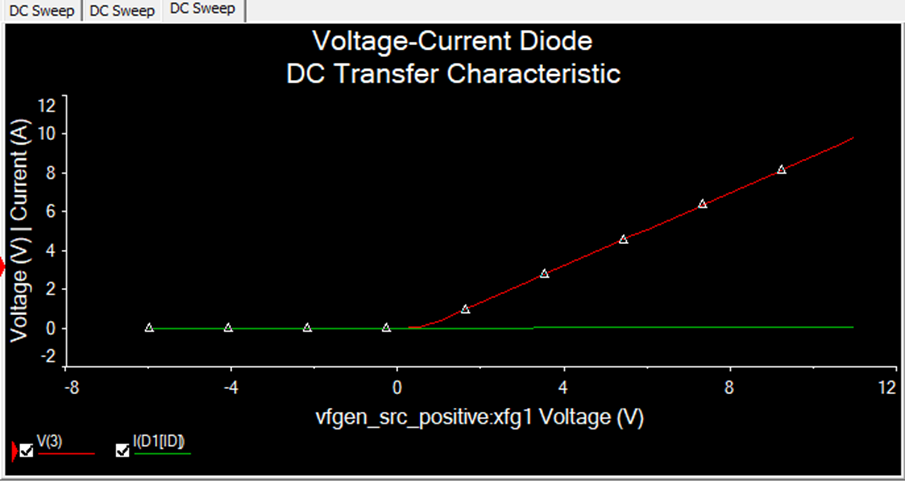
\includegraphics[width=14cm]{vi.png}
    \caption{VI Charecteristics of the Diode}
\end{figure}
	
	{The $V_d$ vs. t waveform for P1(a) had flat peaks at 0.7 V and triangular troughs descending to around -12 V. This is because the diode conducts current when forward-biased, maintaining a constant voltage near its turn-on voltage of 0.7 V. When reverse-biased, it blocks current flow, resulting in a negative triangular shape. The $i_D$ vs. t waveform depicted triangular peaks near 12 V and flat troughs near 0 V, representing current through the diode.}
	
	{Triangular peaks occur when the input voltage exceeds the diode's forward voltage threshold, while flat troughs correspond to reverse-biased conditions. Lastly, the V-I characteristic curve for P1(B) shows minimal current flow at negative Vd values, indicating the diode remains off. At the knee of the curve, the diode begins to conduct, leading to a rapid increase in current, followed by a linear increase, signifying continuous conduction.}

\section{{C2}}

	{Finding $n$;}
	
	$$\because i_D = I_S\left(e^{\frac{V_D}{nV_T} - 1\right)$$
	
	$$\therefore\implies i_{D2} = 2i_{D1}$$
	
	$$\therfore\implies i_{D1} =I_S\left(e^\frac{V_{D2}}{nV_T}\right)$$
	
	$$\therefore i_{D2} = I_S\left(e^\frac{V_{D2}}{nV_T}\right) = I_S\left(e^\frac{V_{D1}}{nV_T}\right)$$
	
	$$\therefore 2\cdot e^\frac{V_{D1}}{nV_T} = e^\frac{V_{D2}}{nV_T}$$
	
	$$\implies \ln{2} = \frac{V_{D2} - V_{D1}}{nV_T}$$
	
	$$\therefore n = \frac{V_{D2} - V_{D1}}{V_{T}\ln{2}} = 1.9826 \approx 1.98$$

\section{{C3}}

	{Error $\% = \left|\frac{\text{Theorectical Value - Measured Value}}{\text{Measured Value}}\right|\cdot 100\%$}

	\begin{table}[H]
    		\centering
    		\begin{tabular}{|c|c|c|c|c|c|}
    		\hline\hline
        		\textbf{$i_D$} [mA] & \textbf{10} & \textbf{7} & \textbf{5} & \textbf{2} & \textbf{1} \\ \hline\hline
        		\textbf{$r_d$ (Theoretical)} & 4.9565 & 7.0807 & 9.913 & 24.7825 & 49.565 \\ \hline
        		\textbf{$r_d$ (Experimental)} & 3.1276 & 6.289 & 7.1146 & 11.7 & 39.52 \\ \hline
        		\textbf{Error Percentage} & 58.476\% & 12.588\% & 39.333\% & 111.816\% & 25.417\% \\ \hline\hline
    		\end{tabular}
	\end{table}

	{Sample Theoretical Value Calculation given that $n \approx 1.9826$ for a $i_D = 10$mA:}

	$$r_d = n\frac{V_T}{i_D} \approx 4.9565$$

\section{{C4}}

	{Results from Table E1 confirm the conventional understanding that the diode voltage rises by approximately 60 nV for every decade increase in current. A sample calculation supports this assertion.}

	{Sample Calculation:}
	
	{At 1 mA, $V_{D1} = 0.6095$ V, Using an n value of 1.9826, derived from \textbf{{C2}}}
	
     $$60 \times 1.9826 = 118.956 \text{mV}$$
     
     $$0.6095 \text{V} + 0.118956 \text{V} = 0.728456 \text{V}$$

	{This calculation substantiates the common understanding, yielding a value of 0.728456 volts, closely resembling the lab's recorded $V_{D1}$ value at 10 mA. Thus, at 1 mA, $V_{D1}$ was 0.6095 volts, while at 10 mA, it rose to 0.728456 volts, affirming the expected increase of about 60 nV.}


